% !TEX root = ./busty_transcription.tex
\section{Beyond Means in Gene Expression}
\label{sec:beyond_means}
 
In this section, our objective is to explore the same models considered in the
previous section, but now with reference to the the question of how well they
describe the distribution of gene expression levels, with special reference to
the variance in these distributions. To that end, we repeat the same pattern as
in the previous section by examining the models one by one. In particular
we will focus on the Fano factor, defined as the variance/mean. This metric
serves as a powerful discriminatory tool from the null model that the
steady-state mRNA distribution must be Poisson, giving a Fano factor of one.

\subsection{A one-state promoter with bursting is the ``best'' model of
constitutive promoters}

Before we can tackle simple repression, we need an adequate phenomenological
model of constitutive expression. The literature abounds with options from which
we can choose, and we show several potential kinetic models for constitutive
promoters in~\fig{fig2:constit_cartoons}. Let us consider the suitability of
each model for our purposes in turn.

\begin{figure}%[h!]
\centering
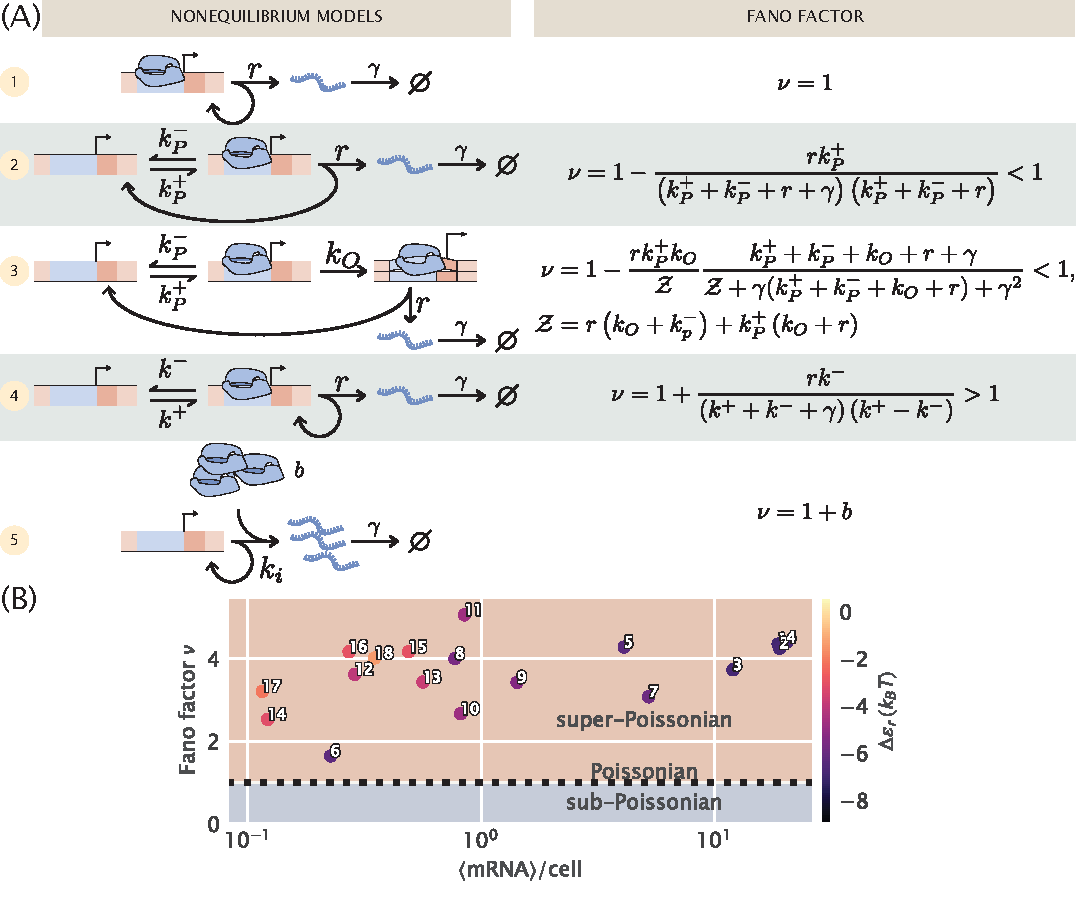
\includegraphics[width=\textwidth]{../figures/main/fig02.pdf}
\caption{\textbf{Comparison of different models for noise in the constitutive promoter.}
(A) The left column depicts various plausible models for the dynamics of
constitutive promoters. In model (1), transcripts are produced in a Poisson
process~\cite{Sanchez2013, Jones2014}. Model (2) features explicit modeling of
RNAP binding/unbinding kinetics~\cite{Phillips2015a}. Model (3) is a more
detailed generalization of model (2), treating transcription initiation as a
multi-step process proceeding through closed and open
complexes~\cite{Mitarai2015}. Model (4) is somewhat analogous to (2) except with
the precise nature of active and inactive states left
ambiguous~\cite{Peccoud1995, Shahrezaei2008, Razo-Mejia2020}. Finally, model (5)
can be viewed as a certain limit of model (4) in which transcripts are produced
in bursts, and initiation of bursts is a Poisson process. 
% \mmnote{Haven't found model 5 formulated quite like this in the literature,
% usually burstiness is handled like model 4, but I should probably search a bit
% more.} 
The right column shows the Fano factor $\nu$ (variance/mean) for each model.
Note especially the crucial diagnostic: (2) and (3) have $\nu$ strictly below 1,
while only for (4) and (5) can $\nu$ exceed 1. Models with Fano factors $\le 1$
cannot produce the FISH data observed in part (B) without introducing
additional assumptions and model complexity. (B) Data from \cite{Jones2014}.
Mean mRNA count vs. Fano factor (variance/mean) for different promoters as
determined with single-molecule mRNA FISH. The colorbar indicates the predicted
binding affinity of RNAP to the promoter sequence as determined in
\cite{Brewster2012}. Numbers serve for cross comparison with data presented in 
Figure 3.}
\label{fig2:constit_cartoons}
\end{figure}

\subsubsection{Noise in the Poisson Promoter Model}

The simplest model of constitutive expression that we can imagine is shown as
model 1 in Figure~\ref{fig2:constit_cartoons} and assumes that transcripts are
produced as a Poisson process from a single promoter state. This is the picture
from Jones et.\ al.~\cite{Jones2014} that was used to interpret a systematic
study of gene expression noise over a series of promoters designed to have
different strengths. This model insists that the ``true'' mRNA distribution is
Poisson, implying the Fano factor $\nu$ must be 1. In~\cite{Jones2014}, the
authors carefully attribute measured deviations from Fano = 1 to intensity
variability in fluorescent spots, gene copy number variation, and copy number
fluctuations of the transcription machinery, e.g., RNAP itself. In this picture,
the master equation makes no appearance, and all the corrections to Poisson
behavior are derived as additive corrections to the Fano factor. For disproving
the ``universal noise curve'' from So et al~\cite{So2011}, this picture was
excellent. It is appealing in its simplicity, with only two parameters, the
initiation rate $r$ and degradation rate $\gamma$. Since $\gamma$ is
independently known from other experiments, and the mean mRNA copy number is
$r/\gamma$, $r$ is easily inferred from data. In other words, the model is not
excessively complex for the data at hand. But for many interesting questions,
for instance in the recent work~\cite{Razo-Mejia2020}, knowledge of means and
variances alone is insufficient, and a description of the full distribution of
molecular counts is necessary. For this we need a (slightly) more complex model
than model 1 that would allow us to incorporate the non-Poissonian features of
constitutive promoters directly into a master equation formulation.

\subsubsection{Noise in the Two-State Promoter, RNAP Bound or Unbound.}

Our second model of constitutive transcription posits an architecture in which
the promoter is either empty or bound by RNAP ~\cite{Phillips2015a,
Phillips2019}. Here,  as shown in model 2 of Figure~\ref{fig2:constit_cartoons},
transcription initiation results in a state transition from the bound to the
unbound state, reflecting the microscopic reality that an RNAP that has begun to
elongate a transcript is no longer available at the start site to begin another.
As shown in Appendix~\ref{sec:non_bursty}, the Fano factor in this model is
given by
\begin{align}
    \nu = 1 -
        \frac{r\rate{k}{P}{+}}
            {\left(\rate{k}{P}{+} + \rate{k}{P}{-} + r\right)
             \left(\gamma + \rate{k}{P}{+} + \rate{k}{P}{-} + r\right)}.
\end{align}
The problem with this picture is that the Fano factor is always $<1$. To make
 contact with the experimental reality of $\nu>1$, clearly some corrections will
 be needed. While this model adds an appealing element of microscopic reality,
 we are forced to reject it as the additional complexity is unable to capture
 the phenomenology of interest. Obviously the promoter state does in fact
 proceed through cycles of RNAP binding, initiating, and elongating, but it
 seems that the super-Poissonian noise in mRNA copy number we want to model must
 be governed by other features of the system.

\subsubsection{Noise in the Three-State Promoter, Multistep Transcription
Initiation and Escape.} 

How might we remedy the deficits of model 2? It is known~\cite{DeHaseth1998}
that once RNAP initially binds the promoter region, a multitude of distinct
steps occur sequentially before RNAP finally escapes into the elongation phase.
Perhaps adding some of this mechanistic detail as shown in model 3 of
Figure~\ref{fig2:constit_cartoons} might rescue the previous model. The next
simplest refinement of that model could consider open complex formation and
promoter escape as separate steps rather than as a single effective step. In
other words, we construct model 3 by adding a single extra state to model 2, and
we will label the two RNAP-bound states as the closed and open complexes,
despite the true biochemical details certainly being more complex. For example,
earlier work extended this model by adding an additional repressor bound state
and did not explicitly consider the limit with no repressor that we analyze
here~\cite{Mitarai2015}. Again, our goal here is not a complete accounting of
all the relevant biochemical detail; this is an exploratory search for the
important features that a model needs to include to square with the known
experimental reality of constitutive expression.

Unfortunately, as hinted at in earlier work~\cite{Mitarai2015}, this model too
has Fano factor $\nu<1$. This can be seen by starting with their Eq.~A1 for the
Fano factor of the analogous model with repressor and taking the limit as
repressor concentration goes to zero. After substantial algebra, the result is
\begin{align}
\nu = 1 - \frac{r k_O k_P^+}{\mathcal{Z}}
\frac{k_P^+ + k_P^- + k_O + \gamma}
        {\mathcal{Z} + \gamma(k_P^+ + k_P^- + k_O + \gamma) + \gamma^2},
\end{align}
where we defined $\mathcal{Z} = r(k_O + k_P^-) + k_P^+(k_O + r)$ for notational
tidiness. This is necessarily less than 1 for arbitrary rate constants.

\marginpar{\it RP: very fun next paragraph - I like the argument, need to think more}
In fact, we suspect \textit{any} model in which transcription proceeds through a
multistep cycle must necessarily have $\nu<1$. The intuitive argument compares
the waiting time distribution to traverse the cycle with the waiting time for a
Poisson promoter (model 1) with the same mean time. The latter is simply an
exponential distribution. The former is a convolution of multiple exponentials,
and intuitively should be more peaked with a smaller fractional width than an
exponential with the same mean.
\footnote{This can be made more precise with a result from~\cite{Stewart2007},
who showed that the convolution of multiple gamma distributions (of which the
exponential distribution is a special case) is, to a very good approximation,
also gamma distributed. Using their Eq.~2 for the distribution of the
convolution, with shape parameters set to 1 to give exponential distributions,
the total waiting time distribution has a ratio of variance to squared mean
$\sigma^2/\mu^2 = \sum_i k_i^2/\left(\sum_i k_i\right)^2$, where the $k_i$ are
the rates of the individual steps. Clearly this is less than 1 and therefore the
total waiting time distribution is narrower than the corresponding exponential.}
A less disperse waiting time distribution means transcription initations are
more uniformly distributed in time relative to a Poisson process. Hence the
distribution of mRNA over a population of cells should be less variable compared
to Poisson, giving $\nu<1$.
\footnote{This last step, while intuitive, can be argued by analogy to photon
statistics where antibunching gives rise to sub-Poissonian noise~\cite{Paul1982,
Zou1990}. Although loopholes exist, we do not expect they apply for our problem.
Nevertheless we refrain from elevating this cycle/sub-Poissonian equivalence to
a ``theorem.'' \mmnote{Antibunching is the ``obvious'' analogy for me but it'd
be totally out of left field for most readers, any suggestions on a more
comprehensible reference??}}

Regardless of the merits of this model in describing the noise properties of
constitutive transcription initiation, it ultimately fails the simplest
quantitative feature of the data, namely that the Fano factor $> 1$ and hence
we must discard this mechanistic picture and search elsewhere.

\subsubsection{Noise in a Two-State Promoter with ``Active'' and ``Inactive''
States}

Inspired by~\cite{Razo-Mejia2020}, we revisit an analog of model 2, but as with
the models considered in \ref{section_02_means}, the interpretation of the two
states is changed. Rather than explicitly viewing them as RNAP bound and
unbound, we view them as ``active'' and ``inactive,'' which are able and unable
to initiate transcripts, respectively. We are noncommittal as to the microscopic
details of these states.

One interpretation~\cite{Chong2014, Sevier2016} for the active and inactive
states is that they represent the promoter's supercoiling state: transitions to
the inactive state are caused by accumulation of positive supercoiling, which
inhibits transcription, and transitions back to ``active'' are caused by gyrase
or other topoisomerases relieving the supercoiling. This is an interesting
possibility because it would mean the timescale for promoter state transitions
is driven by topoisomerase kinetics, not by RNAP kinetics. From in vitro
measurements, the former are suggested to be of order minutes~\cite{Chong2014}.
Contrast this with model 2, where the state transitions are assumed to be
governed by RNAP, which, assuming a copy number per cell of order $10^3$, has a
diffusion-limited association rate $k_{on} \sim 10^2~\text{s}^{-1}$ to a target
promoter. Combined with known $K_d$'s of order $\mu$M, this gives an RNAP
dissociation rate $k_{off}$ of order $10^2$~s$^{-1}$. As we will show below,
however, there are some lingering puzzles with interpreting this supercoiling
hypothesis, so we leave it as a speculation and refrain from assigning definite
physical meaning to the two states in this model.

Intuitively one might expect that, since transcripts are produced as a Poisson
process only when the promoter is in one of the two states in this model,
transcription initiations should now be ``bunched,'' in contrast to the
``anti-bunching'' of models 2 and 3 above. One might further guess that this
bunching would lead to super-Poissonian noise in the mRNA distribution over a
population of cells.  Indeed, as shown in Appendix~\ref{sec:non_bursty}, a
calculation of the Fano factor produces
\begin{align}
\nu &= 1 + \frac{r k^-}{(k^+ + k^- + \gamma)(k^+ + k^-)},
\end{align}
which is strictly greater than 1, verifying the above intuition. Note we have
dropped the $P$ label on the promoter switching rates to emphasize that these
very likely do not represent kinetics of RNAP itself. This calculation can also
be sidestepped by noting that the model is mathematically equivalent to the
simple repression model from~\cite{Jones2014}, with states and rates relabeled
and reinterpreted.

How does this model compare to model 1 above? In model 1, all non-Poisson
features of the mRNA distribution were handled as extrinsic corrections. By
contrast, here the 3 parameter model is used to fit the full mRNA distribution
as measured in mRNA FISH experiments. In essence, all variability in the mRNA
distribution is regarded as ``intrinsic,'' arising either from stochastic
initiation or from switching between the two coarse-grained promoter states. The
advantage of this approach is that it fits neatly into the master equation
picture, and the parameters thus inferred can be used as input for more
complicated models with regulation by transcription factors.

While this seems promising, there is a major drawback for our purposes which was
already uncovered by the authors of~\cite{Razo-Mejia2020}: the statistical
inference problem is nonidentifiable, in the sense described in Section 4.3
of~\cite{Gelman2013}. What this means is that it is impossible to infer the
parameters $r$ and $k^-$ from the FISH data of~\cite{Jones2014} (as shown in
Fig.~S2 of~\cite{Razo-Mejia2020}). Rather, only the ratio $r/k^-$ could be
inferred. In that work, the problem was worked around with an informative prior
on the ratio $k^-/k^+$. That approach is unlikely to work here, as, recall, our
entire goal in modeling constitutive expression is to use it as the basis for a
yet more complicated model, when we add on repression. But adding more
complexity to a model that is already poorly identified is a fool's errand, so
we will explore one more potential model.


\subsubsection{Noise Model for One-State Promoter with Explicit Bursts}

The final model we consider is 
inspired by the failure mode of model 4. The key observation above
was that, as found in~\cite{Razo-Mejia2020}, only two parameters, $k^+$ and the
ratio $r/k^-$, could be directly inferred from the FISH data
from~\cite{Jones2014}. So let us take this seriously and imagine a model where
these are the only two model parameters. What would this model look like?

\marginpar{\it RP: best description I have ever seen of this.  Good job}
To develop some intuition, consider model 4 in the limit $k^+ \ll k^- \lesssim
r$, which is roughly satisfied by the parameters inferred
in~\cite{Razo-Mejia2020}. In this limit, the system spends the majority of its
time in the inactive state, occasionally becoming active and making a burst of
transcripts. This should call to mind the well-known phenomenon of
transcriptional bursting, as reported in,
e.g.,~\cite{Golding2005,Chong2014,Sevier2016}\mmnote{should probably add some
more cites here}. Let us make this correspondence more precise. The mean dwell
time in the active state is $1/k^-$. While in this state, transcripts are
produced at a rate $r$ per unit time. So on average, $r/k^-$ transcripts are
produced before the system switches to the inactive state. Once in the inactive
state, the system dwells there for an average time $1/k^+$ before returning to
the active state and repeating the process. $r/k^-$ resembles an average burst
size, and $1/k^+$ resembles the time interval between burst events. More
precisely, $1/k^+$ is the mean time between the end of one burst and the start
of the next, whereas $1/k^+ + 1/k^-$ would be the mean interval between the
start of two successive burst events, but in the limit $k^+ \ll k^-$, $1/k^+ +
1/k^- \approx 1/k^+$. Note that this limit ensures that the waiting time between
bursts is approximately exponentially distributed, with mean set by the only
timescale left in the problem, $1/k^+$.
\footnote{If instead it were the case that $k^+ \sim k^-$, then the waiting time
$1/k^+ + 1/k^-$ would have a peaked distribution, but this does not appear to be
the case for any of datasets from~\cite{Jones2014}.}

Let us now verify this intuition with a precise derivation to check that $r/k^-$
is in fact the mean burst size and to obtain the full burst size distribution.
Consider first a constant, known dwell time $T$ in the active state. Transcripts
are produced at a rate $r$ per unit time, so the number of transcripts $n$
produced during $T$ fits exactly the ``story'' for the Poisson distribution,
i.e.,
\begin{equation}
    P(n\mid T) = \frac{(rT)^n}{n!} \exp(-rT).
\end{equation}
Since the dwell time $T$ is unobservable, we actually want $P(n)$, the dwell
time distribution with no conditioning on $T$. Basic rules of probability theory
tell us we can write $P(n)$ in terms of $P(n\mid T)$ as
\begin{equation}
    P(n) =\int_0^\infty P(n\mid T) P(T) dT.
\end{equation}
But we know the dwell time distribution $P(T)$, which is exponentially
distributed according to
\begin{equation}
    P(T) = k^- \exp(-T k^-),
\end{equation}
so $P(n)$ can be written as
\begin{equation}
    P(n) = k^- \frac{r^n}{n!}
            \int_0^\infty T^n\exp[-(r + k^-)T]\,dT.
\end{equation}
A standard integral table shows $\int_0^\infty x^n e^{-ax}\,dx = n!/a^{n+1}$, so
\begin{equation}
    P(n) = \frac{k^- r^n}{(k^- + r)^{n+1}}
        = \frac{k^-}{k^- + r}
            \left(\frac{r}{k^- + r}\right)^n
        = \frac{k^-}{k^- + r}
            \left(1 - \frac{k^-}{k^- + r}\right)^n,
\end{equation}
which is exactly the geometric distribution with standard parameter
$\theta\equiv k^-/(k^- + r)$ and domain $n \in \{0, 1, 2, \dots\}$ (this is one
of two common conventions for the geometric distribution). The mean of the
geometric distribution, with this convention, is
\begin{align}
\langle n\rangle = \frac{1 - \theta}{\theta}
        = \left(1 - \frac{k^-}{k^- + r}\right)
                    \frac{k^- + r}{k^-}
        = \frac{r}{k^-},
\end{align}
exactly as we guessed intuitively above.

So in taking the limit $r,k^-\rightarrow\infty$, $r/k^-\equiv b$, we obtain a
model which effectively has only a single promoter state, which initiates bursts
at rate $k^+$ (transitions to the active state, in the model 4 picture). The
master equation for mRNA copy number $m$ as derived in
Appendix~\ref{sec:non_bursty} takes the form
\begin{align}
\begin{split}
{d \over dt}p(m,t) = & (m+1)\gamma p(m+1,t) - m\gamma p(m,t) \\
        &+ \sum_{m'=0}^{m-1} k_i p(m',t) \text{Geom}(m-m';b)
         - \sum_{m'=m+1}^\infty k_i p(m,t) \text{Geom}(m'-m;b),
\end{split}
\end{align}
where we use $k_i$ to denote the burst initiation rate, $\text{Geom}(n;b)$ is the
geometric distribution with mean~$b$, i.e., $\text{Geom}(n;b) =
\frac{1}{1+b}\left(\frac{b}{1+b}\right)^n$ (with domain over nonnegative
integers as above). The first two terms are the usual mRNA degradation terms.
The third term enumerates all ways the system can produce a burst of transcripts
and arrive at copy number $m$, given that it had copy number $m'$ before the
burst. The fourth term allows the system to start with copy number $m$, then
produce a burst and end with copy number $m'$. In fact this last sum has trivial
$m'$ dependence and simply enforces normalization of the geometric distribution.
Carrying it out we have
\begin{equation}
\begin{split}
{d \over dt} p(m,t) = & (m+1)\gamma p(m+1,t) - m\gamma p(m,t) \\
        &+ \sum_{m'=0}^{m-1} k_i p(m',t) \text{Geom}(m-m';b)
            - k_i p(m,t),
\end{split}
\end{equation}
We direct readers again to Appendix~\ref{sec:beyond_means} for further details.
This improves on model 4 in that now the parameters are easily inferred, as we
will see later, and have clean interpretations. The non-Poissonian features are
attributed to the empirically well-established phenomenological picture of
bursty transcription.

The big approximation in going from model 4 to 5 is that a burst is produced
instantaneously rather than over a finite time. If the true burst duration is
not short compared to transcription factor kinetic timescales, this could be a
problem in that mean burst size in the presence and absence of repressors could
change, rendering parameter inferences from the constitutive case inappropriate.
Let us make some simple estimates of this.

Consider the time delay between the first and final RNAPs in a burst initiating
transcription (\textit{not} the time to complete transcripts, which potentially
could be much longer.) If this timescale is short compared to the typical search
timescale of transcription factors, then all is well. The estimates from
deHaseth et.\ al.~\cite{DeHaseth1998} put RNAP's diffusion-limited on rate
around $\sim\text{few}\times10^{-2}~\text{nM}^{-1}~\text{s}^{-1}$ and polymerase
loading as high as $1~\text{s}^{-1}$. Then for reasonable burst sizes of $<10$,
it is reasonable to guess that bursts might finish initiating on a timescale of
tens of seconds or less (with another 30-60 sec to finish elongation, but that
does not matter here). A transcription factor with typical copy number of order
10 (or less) would have a diffusion-limited association rate of order
$(10~\text{sec})^{-1}$ \mrm{cite Elf?}. Higher copy number TFs tend to have many
binding sites over the genome, which should serve to pull them out of
circulation and keep their effective association rates from rising too large.
Therefore, there is \textit{perhaps} a timescale separation possible between
transcription factor association rates and burst durations, but this assumption
could very well break down, so we will have to keep it in mind when we infer
repressor rates from the Jones et.\ al.\ FISH data later~\cite{Jones2014}.

In reflecting on these 5 models, the reader may feel that exploring a multitude
of potential models just to return to a very minimal phenomenological model of
bursty transcription may seem highly pedantic. But the purpose of the exercise
was to examine a host of models from the literature and understand why they are
insufficient, one way or another, for our purposes. Along the way we have
learned that the detailed kinetics of RNAP binding and initiating transcription
are probably irrelevant for setting the population distribution of mRNA. The
timescales are simply too fast, and as we will see later
in~\fig{fig:constit_post}, the noise seems to be governed by slower timescales.
Perhaps in hindsight this is not surprising: intuitively, the degradation rate
$\gamma$ sets the fundamental timescale for mRNA dynamics, and any other
processes that substantially modulate the mRNA distribution should not differ
from $\gamma$ by orders of magnitude.